\documentclass[a4paper,12pt]{article}
\usepackage[utf8]{inputenc}
\usepackage{url}
\usepackage{epsfig}
\usepackage{graphics}
\usepackage{fancyhdr}
\usepackage{subfig}
\usepackage{subfiles}
\usepackage{booktabs}

\graphicspath{{pictures/}}
\begin{document}

\title{Sentence Generation using Two Models \\ \large{Project in the course DD2380 at KTH}}

\author{
Group 61\\ \\[0.05cm]
\begin{tabular}{cccc}
K. Hannesson & J. Jóhannsson & E. Ahlsén & J. Andersson\\
\normalsize{August 20} & \normalsize{January 12} & \normalsize{February 9} & \normalsize{February 10} \\
\normalsize{1982} & \normalsize{1984} & \normalsize{1988} & \normalsize{1984} \\
{\normalsize hannesso@kth.se} & {\small jokull@kth.se} & {\small edvarda@kth.se} & {\small jonand8@kth.se} \\ \\[0.05cm]
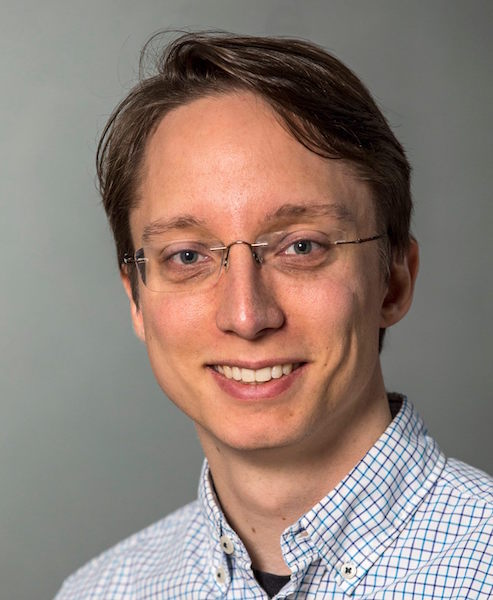
\includegraphics[width=0.13\linewidth]{photo_Kristofer} &
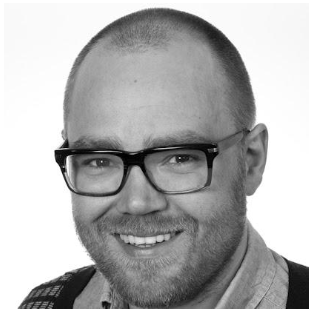
\includegraphics[width=0.13\linewidth]{photo_Jokull} &
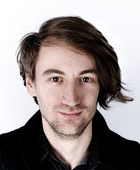
\includegraphics[width=0.13\linewidth]{photo_Edvard} &
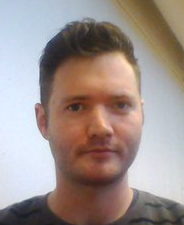
\includegraphics[width=0.13\linewidth]{photo_Jonas}
\\[0.7cm]
\end{tabular}
}

% Normally there will not be any pictures but we want
% these so that we can connect faces to names in the course
% We also want birthdates so that we can tell people with the same
% name apart
\date{\today}

\pagestyle{fancy}
\setlength{\headheight}{15pt}
\fancyhf{}
\lhead{DD2380 ai15} % DO NOT REMOVE!!!!
\rhead{K. Hannesson, J. Jóhannsson, E. Ahlsén, J. Andersson} %% UPDATE WITH YOUR NAMES
\fancyfoot[C]{\thepage}



\maketitle
\thispagestyle{fancy}

\begin{abstract}
In this paper, two different approaches to constructing n-gram models for Natural Language Generation (henceforth NLG) are discussed and contrasted. Our main focus was creating text that would qualify as human generated. We also investigate how different types of smoothing techniques impact the performance of the models. The two models were evaluated via a perception test in the form of an online survey. Unfortunately, errors were identified after the survey was administered, which effectively make the results inconclusive in predicating anything about our models.
\end{abstract}



\clearpage

%%%%%%%%%%%%%%%%%%%%%%%%%%%%%%%%%%%%%%%%%%%%%%%%%%%%%%%%%%%%%
%%%%%%%%%%%%%%%%%%%%%%%%%%%%%%%%%%%%%%%%%%%%%%%%%%%%%%%%%%%%%
%\section*{NOTE}
%\begin{itemize}
%
%\item The following sections are arranged in the order they would appear in a scientific paper. We think that these sections need to be there and written. However, these are only guidelines and if you think that some of these sections or subsections are irrelevant to you, please feel free to remove them. Similarly, if you want to include more sections or subsections please go ahead. Also feel free to rearrange them according to your convenience, but keeping some common sense (eg.~Introduction cannot come after Conclusions).
%
%\item \textit{Introduction, Related Works, Experimental Results, Discussions, Summary} are sections that MUST be contained.
%
%\item In the section of your \textit{Method}: please do not list your project as log book entries, please talk about the final method you want to present to us. Talk about the method scientifically or technically and not as "I did this..." "Then I tried this..." "this happened...." etc.
%
%\item Do not paste any code unless it is very relevant!
%
%\item The section \textit{Contributions} is a place to express any difference in contributions. The default assumption is that you all agree that all of you had an equal part to play in the project.
%
%\item We suggest that you try to write this as scientifically as possible and not simply like a project report. Good Luck!
%
%\item Please remove \textbf{this} NOTE section in your final report.
%
%\end{itemize}
\section{Introduction} %(1--2 pages)
\label{sec:intro}

\subfile{introduction}

%**
%Why was the study undertaken? What was the research question, the tested hypothesis or the purpose of the research?
%**


\section{Outline}
Beginning in \ref{sec:relwork}, we start off by briefly describing how our project relates to other projects in the field from which we gathered inspiration, and what we learned and applied from those. \ref{sec:method} details the characteristics of our proposed models, and hypothesizes about their functionality. It also contains a brief introduction to the different smoothing techniques employed. \ref{sec:exps}, the design and outcome of the experiment is accounted for, and in \ref{sec:summary} we try to summarize the results of our work. Finally, \ref{sec:contributions} recounts the contributions of the different members of the team to the project.


%%%%%%%%%%%%%%%%%%%%%%%%%%%%%%%%%%%%%%%%%%%%%%%%%%%%%%%%%%%%%
%%%%%%%%%%%%%%%%%%%%%%%%%%%%%%%%%%%%%%%%%%%%%%%%%%%%%%%%%%%%%
\section{Related work}
\label{sec:relwork}

\subfile{related_works}

%%%%%%%%%%%%%%%%%%%%%%%%%%%%%%%%%%%%%%%%%%%%%%%%%%%%%%%%%%%%%
%%%%%%%%%%%%%%%%%%%%%%%%%%%%%%%%%%%%%%%%%%%%%%%%%%%%%%%%%%%%%
\section{Our method}
\label{sec:method}

The group came up with the idea to compare two different approaches to generating text from a corpus, both including grammar but in different ways. To be able to compare them at the same level both approaches used the Brown corpus and trigrams, with fallback to bigrams allowed. A few smoothing techniques were picked for use in both approaches.

\subsection{Sentence generation}
The same general method for word generation was used for both of the models; after coming up with a probability distribution for the next word, which is done differently in each of the models, a random word would be picked from the distribution, where the probability of a word being picked is equal to that words probability in the distribution.


\subsection{Semantic model}
The first approach was to create a model that included both word and grammar information. This was achieved by generating trigrams where each word was a tuple of the word and its associated Part-Of-Speech (POS) tag. A trigram from ``the man walked'' would be (the, DET), (man, NOUN), (walked, VERB))

The distribution table contains the n-1-gram plus the tags as a key and the distribution probability of the next word. In the example above the key would be (the, DET), (man, NOUN) and that row in the table would contain the probability distribution of each word and tag that could follow that word given the corpus.

To be able to use fallback each model had 2-grams up to n-grams models. If a word/tag was not found using the n-gram model we would fallback to the n-1-gram model and so forth.

To be able to distinguish words that are in the beginning of sentence and in the end of sentence we added pseudo symbols to each sentence. The number of symbols added to the start and end of sentence would correspond n-1 in the model. Meaning that 2 start symbols were added to a trigram model.

\subsubsection{Hypothesis}
The Semantic model aims at modeling chains of sense-disambiguated words by building a model of (word,POS-tag) tuples from a tagged corpus. The idea is to constrain the sense in which a word is used to the word-senses of the preceding words. Using word-senses effectively expands the size of the vocabulary by a factor equal to the average number of different POS-tags for an average word in the corpus. This leads to more sparse data in the model, compared to modeling words by themselves, but it should also eliminate a lot of problems with semantic disagreement in the generated text.

\subsection{Inferred grammar model}
The second approach separated grammar and words into two models which were used in sequence to generate text. The grammar model was built using sentences of POS-tags from a tagged corpus, while the word-grammar model was built using both words and tags. The grammar model would generate a likely next tag based upon the previous tags, which the word model would then use as a constraint for selecting the next word. In terms of data structures, this made the model look like an n+1 order model as compared to the grammar model, but without increasing the number of preceding words that a new word depended on, but instead constraining it to a specific grammatical tag.
The grammar model generates tag by looking at $P(t_3|t_1,t_2)$, and the word-grammar model then generates words by looking at $P(w_3|w_1,w_2,t_3)$.

\subsubsection{Hypothesis}
The idea behind the Inferred grammar model the grammatical structure of sentences separately from the words in the sentences, allowing any semantically disambiguated words (word/tag tuples) with no collocations in the training set to appear next to each other as long as they satisfy the constraints imposed by the grammar-model trained on the same training set. This, we theorize, will allow for a greater branching factor for the word generation, and thus a greater variance in the sentences produced, without sacrificing much of the grammatical-agreement qualities.

Since the vocabulary of POS-tags is much smaller than the vocabulary of the words in the the training-set, the data for the grammar model will be much more dense.

\subsection{Smoothing}
\label{subsec:smoothing}

The problem with using only Maximum Likelihood Estimation is that it maximises the likelihood to generate the training set. Since the training set is limited in scope, our n-gram models will suffer from sparse data in the sense that a lot of n-grams only occur once or a few times in the training set. MLE will assign them a very low probability, even though they might be perfectly reasonable n-grams to build sentences upon. We chose three different smoothing techniques besides MLE for testing our models.

\subsubsection{Laplace smoothing}
Laplace smoothing works simply by increasing the count of every n-gram by one, before calculating the MLE values, thus effectively redistributing a chunk of the probability mass from the more frequent n-grams to the less frequent ones.

\subsubsection{Expected Likelihood Estimate}
Expected Likelihood Estimate, or 'add-delta', is a variation of Laplace smoothing, that only increases the count of all n-grams by a fraction between 0 and 1. This is to counter the effect of Laplace smoothing where a large chunk of the probability mass would get redistributed if the model has a high ratio of low-count n-grams to high-count n-grams.

\subsubsection{Simplified Good-Turing Frequency Estimation}
\subfile{smoothing-goodturing}

\subsection{Implementation}
\label{sec:impl}

We split into pairs with each pair implementing their model. We decided to go with Python 3 for the implementation because we knew the NLTK package would provide us with the necessary building blocks to construct and test the two models. These included
\begin{itemize}
\item Brown corpus
\item Treebank Part of Speech Tagger (Maximum entropy)
\item Punkt Tokenizer Models
\item Mappings to the Universal and Brown Part-Of-Speech Tagset
\item Conditional Frequency Distribution and Conditional Probability Distribution classes
\item Classes for each of the above mentioned smoothing techniques
\end{itemize}

\subsubsection{Deviations from the plan}
Our implementations unfortunately failed to conform to the specifications we had outlined. The next section outlines how the implemented models deviated from the plan and how the experiment was affected.


%%%%%%%%%%%%%%%%%%%%%%%%%%%%%%%%%%%%%%%%%%%%%%%%%%%%%%%%%%%%%
%%%%%%%%%%%%%%%%%%%%%%%%%%%%%%%%%%%%%%%%%%%%%%%%%%%%%%%%%%%%%
\section{Experimental results}
\label{sec:exps}

\subsection{Models used in experiment}
The models used in the experiments, we later realized, were implemented in a way that was inconsistent with the specifications outlined in {Inferred grammar model}. This was a big setback, since it effectively meant that the data gathered from the experiment told us nothing about the hypothetical models outlined in \ref{sec:method}.

We will use SM* and IGM* to refer to the implementation of the Semantic model and Inferred grammar model used in the experiment.

\subsubsection{Semantic model}
The SM* model was inconsistent with the specifications in that even though the model provides a word along with its tag, these tags were not used for subsequent word generation. Instead the most recent two words were sent in and a POS tagger to determine tags. Sometimes the POS tagger did not generate the correct tag and this resulted in the generated results being inconsistent with the actual tag in the corpus.

\subsubsection{Inferred grammar model}
The implementation of the Inferred grammar model (IGM*) was, among the two experimental models, the one most inconsistent with the specifications.

IGM* separated grammar and words into two models which were used in sequence to generate text. The grammar model, using trigrams of POS-tags, was consistent with our specifications. The word-grammar model generated a new word conditioned upon the previous two POS-tags generated by the grammar model. This is inconsistent with the specifications. For example, IGM* would take ``the man walked'' and create the trigrams (DET, NOUN, VERB) for the grammar model, and (DET, NOUN, walked) for the grammar-word model.

More formally, IGM generates $(w_3|w_1,w_2,t_3)$, while IGM* generates $(w_3 | t_1,t_2)$.

\subsection{Experiment setup}
\label{sec:expiremental_setup}
Model performances were measured using a perception test in the form of an online survey with 30 questions. Both models were used to generate 3 sentences for each of the 4 smoothing methods.  Additionally 3 sentences were hand-picked from the Brown corpus and 3 sequences of random words generated to serve as the ``human'' and ``baseline'' models against which our models would be compared. Each group of 3 was picked by generating a few hundred sentences and picking the top 3 with the best perplexity score. The number of sentences was limited to 30 to avoid testing the patience of the survey participants.

Participants were asked to rate on a scale of 1-5 how closely they felt the sentences resembled human writing. As a guideline they were told that if a sentence appeared to be random words it might receive a 1, if it showed some signs of coherence it might receive a 3, and if it looked like a person wrote it then it would receive a 5. To make the test as fair as possible the sentences were presented to each participant in a random order. The survey platform used was Google Forms and the results where pulled into R for processing and graphical representation.

\begin{figure}
  \centering
    \subfloat[Performance of each model as well as the human and baseline sentences]
    {{\label{fig:hist1}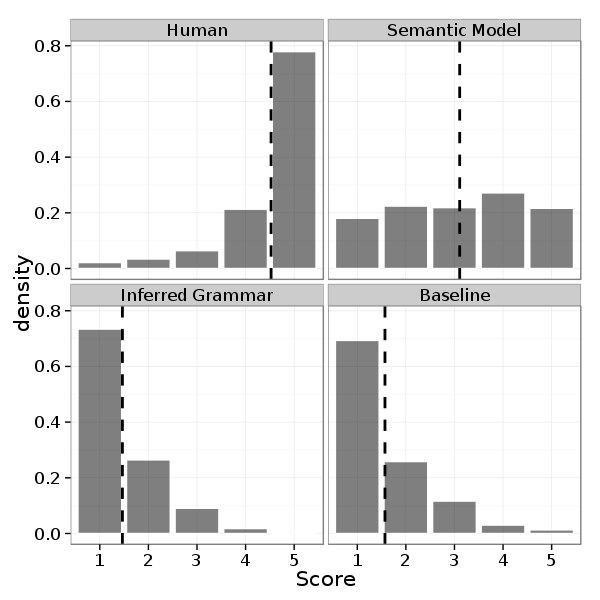
\includegraphics[height=5cm]{results/histogram_resultsByModel}
    }}%
    \qquad
    \subfloat[Performance of each model and smoothing method]{{\label{fig:hist2}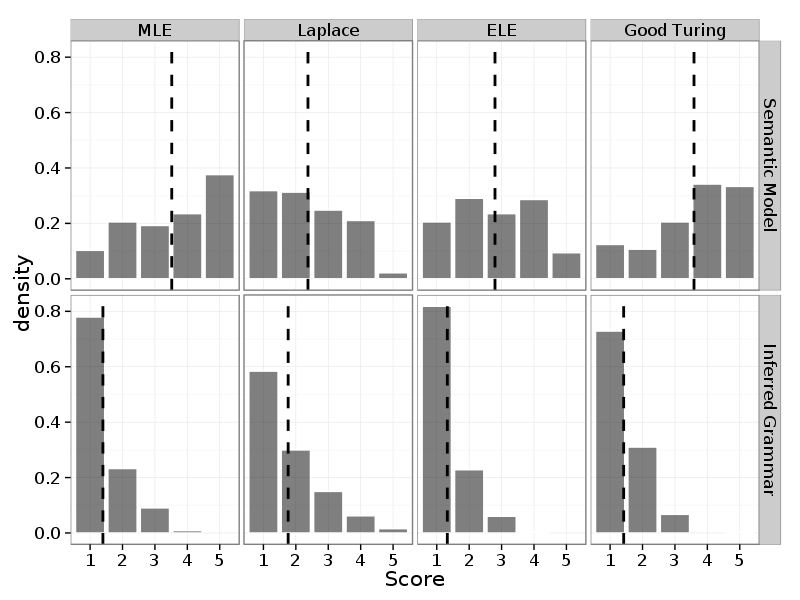
\includegraphics[height=5cm]{results/histogram_resultsByModelAndSmootingMethod}
    }}%
    \caption{Density histograms of model scores in the perception test. Dotted lines represent means.}%
    \label{fig:histograms}%
\end{figure}

\begin{figure}%
    \centering
    \subfloat[Performance of each model as well as the real and baseline sentences]{{\label{fig:boxplot1}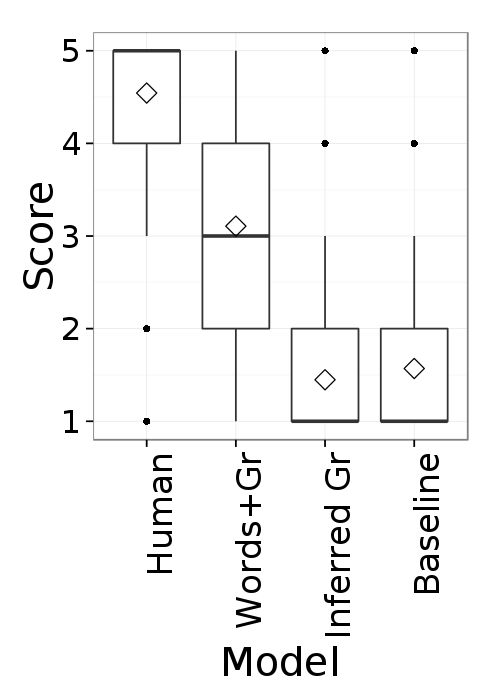
\includegraphics[height=6.2cm]{results/boxplot_resultsByModel} }}%
    \qquad
    \subfloat[Performance of each model and smoothing method]{{\label{fig:boxplot2}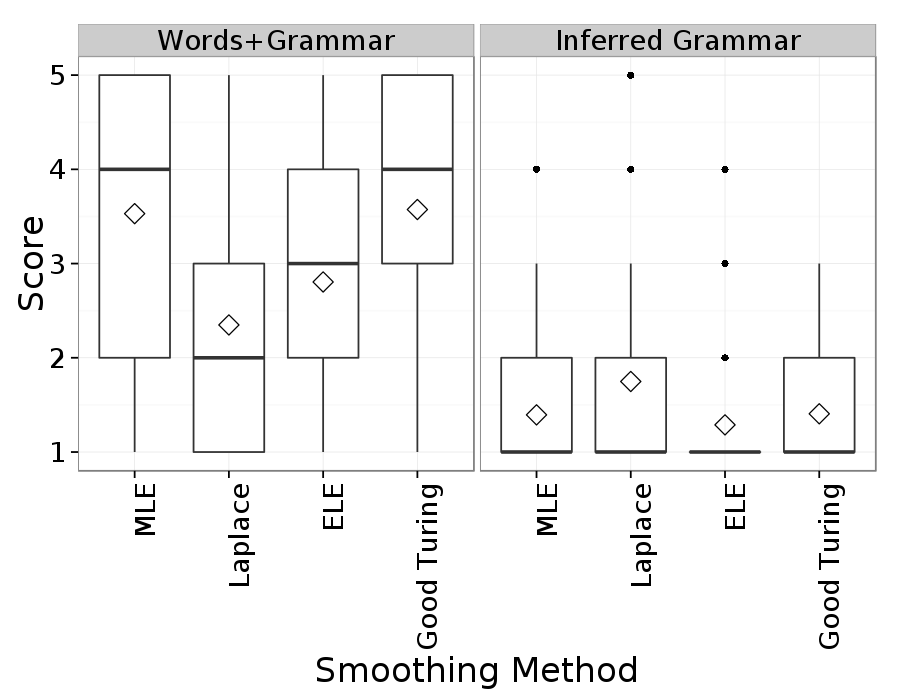
\includegraphics[height=6cm]{results/boxplot_resultsByModelAndSmoothing} }}%
    \qquad
    \caption{Boxplots of model scores in the perception test. Diamonds represent   means.}%
  \label{fig:boxplots}
\end{figure}

\begin{table}[]
\centering
\caption{Model performance statistics from perception test}
\label{tab:modelStats}
\begin{tabular}{@{}lllll@{}}
\toprule
Model            & Smoothing Method & Mean & Median & Mode \\ \midrule
Semantic Model   & MLE              & 3.5  & 4      & 5    \\
Semantic Model   & Laplace          & 2.4  & 2      & 1    \\
Semantic Model   & ELE              & 2.8  & 3      & 2    \\
Semantic Model   & Good Turing      & 3.6  & 4      & 4    \\
Inferred Grammar & MLE              & 1.4  & 1      & 1    \\
Inferred Grammar & Laplace          & 1.8  & 1      & 1    \\
Inferred Grammar & ELE              & 1.3  & 1      & 1    \\
Inferred Grammar & Good Turing      & 1.4  & 1      & 1    \\ \bottomrule
\end{tabular}
\end{table}

%%%%%%%%%%%%%%%%%%%%%%%%%%%%%%%%%%%%%%%%%%
%%%%%%%%%%%%%%%%%%%%%%%%%%%%%%%%%%%%%%%%%%
\subsection{Results}
\label{sec:results}
The results for the two implemented models, as detailed in section~\ref{sec:method}, were very different. The density distribution of answers can been seen in figures~\ref{fig:hist1} and~\ref{fig:hist2} which show that the results for SM* are somewhat uniform while the results for IGM* are are positively skewed with most scores very low. The scores of the human and baseline sentences are positively skewed and negatively skewed, respectively. These are expected results for the baseline and gold-standard. The performance differences become even clearer in figure~\ref{fig:histograms} where we see that IGM* performs no better than the baseline, in fact the baseline has a higher mean score. Looking at the performance of different smoothing methods in figure~\ref{fig:hist2} we see that the Laplace and ELE smoothing methods result in poorer performance than MLE and Simple Good-Turing. MLE and Simple Good-Turing perform very similarly, but the Simple Good-Turing distribution is densest in the 4 and 5 scores while MLE has a greater spread. Simple Good-Turing has the best performance according to the perception test.

The IGM* model perform no better than the randomly generated sentences provided by the baseline no matter the smoothing method, with only Laplace smoothing pulling the mean score slightly up.

%%%%%%%%%%%%%%%%%%%%%%%%%%%%%%%%%%%%%%%%%%%%%%%%%%%%%%%%%%%%%
%%%%%%%%%%%%%%%%%%%%%%%%%%%%%%%%%%%%%%%%%%%%%%%%%%%%%%%%%%%%%


%%%%%%%%%%%%%%%%%%%%%%%%%%%%%%%%%%%%%%%%%%%%%%%%%%%%%%%%%%%%%
%%%%%%%%%%%%%%%%%%%%%%%%%%%%%%%%%%%%%%%%%%%%%%%%%%%%%%%%%%%%%
\section{Summary and Conclusions}
\label{sec:summary}

\subfile{conclusion}
%%%%%%%%%%%%%%%%%%%%%%%%%%%%%%%%%%%%%%%%%%%%%%%%%%%%%%%%%%%%%
%%%%%%%%%%%%%%%%%%%%%%%%%%%%%%%%%%%%%%%%%%%%%%%%%%%%%%%%%%%%%
\section{Contributions}
\label{sec:contributions}
In the beginning of the project all team members agreed that we will always work on the project together. For 5 consecutive weekends in a row the team had a NLP workshop. We started each morning with a meeting to plan  the course of our day. We than splitted up into groups of two. All team members had an equal play in the project.

%%%%%%%%%%%%%%%%%%%%%%%%%%%%%%%%%%%%%%%%%%%%%%%%%%%%%%%%%%%%%
%%%%%%%%%%%%%%%%%%%%%%%%%%%%%%%%%%%%%%%%%%%%%%%%%%%%%%%%%%%%%
\clearpage
\bibliographystyle{plain}
\bibliography{reflist}
\end{document}
